\documentclass[conference]{IEEEtran}
\IEEEoverridecommandlockouts%
\usepackage{cite}
\usepackage{amsmath,amssymb,amsfonts}
\usepackage{algorithmic}
\usepackage{graphicx}
\usepackage{textcomp}
\usepackage{xcolor}
\def\BibTeX{{\rm B\kern-.05em{\sc i\kern-.025em b}\kern-.08em
    T\kern-.1667em\lower.7ex\hbox{E}\kern-.125emX}}
\begin{document}

\title{La física de transistores de película delgada con silicio amorfo}

\author{\IEEEauthorblockN{1\textsuperscript{st}MARTIN J. POWELL}
\IEEEauthorblockA{\textit{dept (of Aff.)} \\
\textit{name of organization (of Aff.)}\\
City, Country \\
email address or ORCID}}

\maketitle

\begin{abstract}
    Los transistores de película delgada de silicio amorfo son importantes
    dispositivos electrónicos que son usados en un amplio rango de aplicaciónes
    en el area de electronica. La física básica subyacente a su funcionamiento
    y los problemas clave de rendimiento se analizan aquí. Las
    características estáticas de los transistores son determinadas por la localización
    de estados electrónicos que ocurren en el bandgap de silicio amorfo.
    Los estados profundos, consisten principalmente en enlaces sueltos de
    Si, esto sirve para determinar el voltaje de umbral y determinar los estados de cola
    del bandgap en la banda de conducción y determinar la movilidad de efecto de campo. 
    Los tiempos finitos de captura y emisión de los estados
    localizados profundos conducen a una característica dinámica del transistor
    que puede describirse mediante un voltaje de umbral dependiente del
    tiempo. 
    \\
    Los transistores también muestran cambios de voltaje de umbral
    con respecto a tiempo más largos debido a otros dos mecanismos distintos; 
    a saber, la captura de carga en el aislante de compuerta de nitruro de silicio y la
    creación de estados de enlaces colgantes metaestables en el silicio amorfo. Estos
    dos mecanismos muestran características diferentes por polarización,
    temperatura, y las dependencia del cambio de voltaje de umbral. La iluminación de 
    los TFT`s causa una generación de pares electron-hueco, en la
    region de carga espacial lo que lleva a un flujo igual de estados estacionarios
    de electrones, huecos y una reducción en la flexion de la banda. En la
    mayoría de aplicaciones, la foto-sensibilidad podría ser minimizada. 
    \\
    Esto se puede hacer disminuyendo el grosor de la capa-$i$, que es más eficaz en
    los TFT`s que utilizan un aislante superior de nitruro de silicio adicional.
    La interfaz superior tiene una alta densidad de centros de recombinación,
    los cuales matan la foto-sensibilidad con una degradación minima de las
    características de transferencia. Las capas de pasivación depositadas sobre
    los TFT`s pueden afectar las características del transistor, si la capa
    de pasivación esta en contacto directo con la capa de silicio amorfo. El
    efecto consecuente sobre las características de transistores depende sobre
    el grosor de las capas. La uniformidad de arreglos grandes de transistores
    para aplicaciones de pantalla es excelente, con variaciones en el voltaje
    de umbral de 0.5 to 1.0V. El rendimiento de los dispositivos también es
    bueno, pero se necesitan más mejoras para la reducción de costes y las
    aplicaciones de mayor tamaño.
\end{abstract}

\begin{IEEEkeywords}
component, formatting, style, styling, insert
\end{IEEEkeywords}

\section{Introduccción}
    Transistores de película delgada de silicio amorfo fueron propuestos como dispositivos
    aplicables por LeComber et al. [1] en 1979. Desde entonces, ha
    habido una enorme actividad, en todo el mundo, que ha dado lugar a la utilización 
    de estos dispositivos en una variedad de aplicaciones. Quizás el mejor
    ejemplo es la matriz activa dirigido a pantallas de cristal liquido, El cual ha sido
    propuesto por mas de 20 compañías y ha liderado, en algunos casos, productos
    comerciales (para un resúmen de estas actividades se pueden ver [2]). Otras aplicaciones
    importantes incluidas de arreglos lineales de sensores de imagen para
    lectores de caras y arreglos lineales para el manejo nuevas impresoras de pagina
    amplia [4]. En todas estas aplicaciones, un minucioso entendimiento de la física
    básica subyacente la operación y el desempeño de los transistores de película
    delgada es esencial, y esto es el objetivo de este articulo. En artículos previos
    [5], el autor describe la relación del desempeño de las propiedades básicas de los
    materiales. Este articulo cubre terreno similar, concentrándose en los temas en
    los que se han producido avances desde 1984.

\section{Tecnologías TFT}
    Los transistores de película delgada de silicio amorfo puede ser hechos con una amplia
    variedad de estructuras y materiales. Básicamente, existen cuatro tipos
    de TFT`s (figura~\ref{fig1}.) Estos definidos por el orden del deposito de las capas, tales como el semiconductor,
    aislante de compuerta, contactos drenaje-fuente, y el electrodo de
    compuerta. Las estructuras escalonadas de los TFt`s tienen los contactos de fuente y drenaje
    sobre un lado del semiconductor y del electrodo de contacto sobre el lado opuesto,
    mientras las estructuras coplanar tienen los tres electrodos sobre
    el mismo lado de la película semiconductora. En la estructura ``invertida'' el
    electrodo de compuerta es la primera capa depositada sobre sustrato de vidrio.
    Los transistores de película delgada de silicio amorfo han realizado con cuatro estructuras,
    pero para todos los datos de los dispositivos usados en aplicaciones
    practicas usan una estructura escalonada. Este contraste para los TFT`s de silicio
    policristalino, los cuales son usualmente una estrcutura coplanar, que es el análogo 
    a transistores MOS de silicio cristalino.
    \\
    Para TFT de silicio amorfo, la estructura mas popular y una de las mas responsables
    para el estado del arte con respecto al desempeño, es el escalonado invertido, el
    cual usa nitruro de silicio como aislante de compuerta [7]. En este articulo, nos
    concentramos sobre este tipo de TFT, todos los resultados obtenidos y discutidos
    sobre este tipo de transistor. Ademas, la física de algunos tópicos es generalmente
    aplicable para algún tipo de TFT de silicio amorfo.

\begin{figure}[htbp]
    \centerline{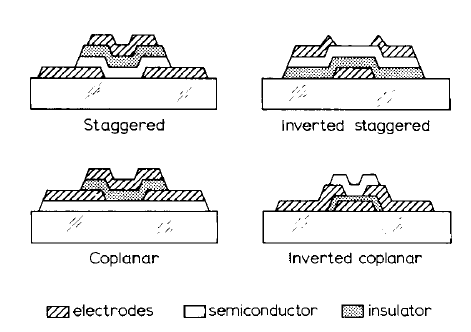
\includegraphics[width=7cm]{img/imagen-1.png}}
    \caption{Example of a figure caption.}%
    \label{fig1}
\end{figure}
 
    Incluso limitándonos al TFT de escalonamiento invertido, hay muchas tecnologías 
    de TFT`s diferentes. La figura~\ref{fig2}, muestra dos tipos de estructuras de TFT`s
    escalonadas invertidas para silicio amorfo el cual ha sido investigado en nuestro
    laboratorio [8]. Las características más comunes de estos TFT`s son el uso de Cr como
    metal para el electrodo de compuerta, como aislante de compuerta nitruro de
    silicio, y la doble capa de metalización Cr/Al para los contactos fuente drenaje.
    La diferencia esencial es el orden de deposito de otras capas. En el tipo A
    existen TFT`s de un deposito consecutivo de nitruro de compuerta, silicio amorfo
    intrínseco, silicio amorfo $n^+$ en un solo paso de crecimiento. El $n^+$ se graba en
    la región del canal del transistor. En el caso del TFT de tipo B, existe un deposito
    consecutivo de nitruro para la compuerta, silicio amorfo intrínseco, y después
    la segunda capa de nitruro de silicio. El nitruro encima es grabado desde las
    regiones de contacto, antes de depositar la capa de $n^+$.

\begin{figure}[htbp]
    \centerline{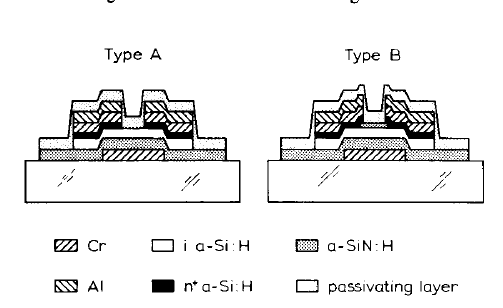
\includegraphics[width=6.0cm]{img/imagen-2.png}}
    \caption{Example of a figure caption.}%
    \label{fig2}
\end{figure}

    Estos tipos de TFT`s han sido investigados por numerosos grupos. Además, todavía 
    hay diferencias en los detalles de la tecnología utilizada por cada grupo.
    Las variaciones incluyen diferentes esquemas de metalización, la posición de
    electrodo transparente, y la adición de una capa de protección ligera o un condensador
    de almacenamiento. El tipo de TFT B requiere un mínimo de tres
    pasos de mascara y el tipo B un mínimo de cuatro pasos de mascaras, pero
    algunas variaciones anteriores pueden aumentar la complejidad del proceso a
    seis o incluso ocho pasos de mascaras.

\section{Características Estaticas del transistor}
   
    Las figuras 3 y 4 muestran ejemplos de las características básicas de 
    transferencia estática y de salida de un transistor de película delgada de silicio 
    amorfo de tipo A, fabricado en nuestro laboratorio. Las características
    de un transistor de tipo B son esencialmente las mismas (q.V). En la figura 3, 
    la aplicación de un voltaje de compuerta que conduce a un aumento aproximadamente 
    exponencial de la corriente de drenaje de origen, al principio, seguido de un 
    aumento lineal de la corriente a tensiones de compuerta mas alta. Para la mayoría 
    de los transistores, observamos una región lineal razonablemente bien definida, 
    que nos permite definir el voltaje de umbral (la intercepción menor a $V_D/2$) 
    y la movilidad de efecto de campo (dada por $\mu_{FE}=(d_{ins}L/ \varepsilon V_d W)(dI_D/dV_G)$)
    donde $dI_D/dV_G$es la pendiente. Los voltajes de umbral tipicos estan en un ragno de $2-4V$
    y las movilidades estan en un rango $0.4- 1.0 cm^2V^{-1}s^{-1}$[7]. El ejemplo se muestra en la figura 3 que 
    tiene una movilidad de $0.6 cm^2V^{-1}s^{-1}$.

\begin{figure}[htbp]
    \centerline{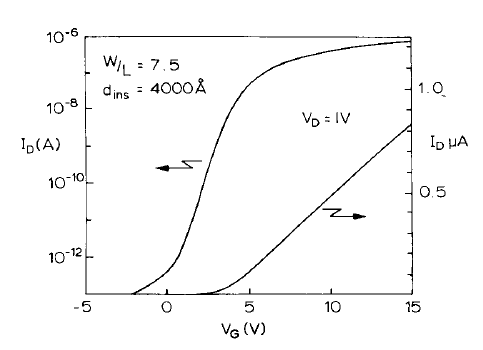
\includegraphics[width=6.0cm]{img/imagen-3.png}}
    \caption{Example of a figure caption.}%
    \label{fig3}
\end{figure} 


\begin{figure}[htbp]
    \centerline{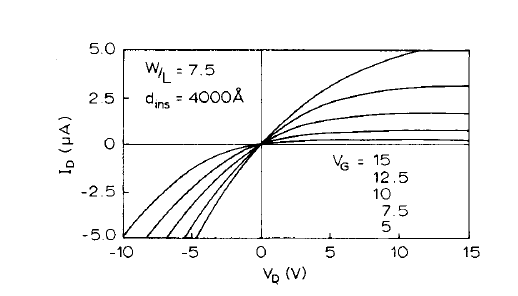
\includegraphics[width=6.0cm]{img/imagen-4.png}}
    \caption{Example of a figure caption.}%
    \label{fig4}
\end{figure} 

    Las características de salida muestran una buena saturación y pueden describirse
    razonablememnte bien mediante las ecuaciones estándar de los MOSFET para las características
    de umbral anteriores. La movilidad de efecto de campo también puede deducirse de la region 
    de saturación mediante el trazado de la raíz cuadrada de la corriente fuente-drenaje
    versus al voltaje de compuerta. Esto da el mismo valor que el deducido de la region lineal, dentro del 
    error experimental. 
    \\
    Una observación importante es la ausencia del estrechamiento de corriente en las
    características de salida [15]. Esto es cierto tatnto para los transistores de 
    tipo A como para los de tipo B y demuestra que la interfaz entre las capas $n^+$ e $i$
    puede ser de calidad suficiente en las dos tecnologías, aunque el transistor de tipo B 
    tenga un deposito interrumpido. La ausencia de aglomertación de corriente (current crowding),
    signiofica que la densidad de estados es menor en la masa de a-Si:H que en la región de a-Si:H
    cerca de la interfaz de compuerta [5][15].
    El funcionamiento basico del transistor puede entenderse por la refernecia en la figura 5, 
    donde ilustramos esquemáticamente la flexión de banda y la ocupación de los estados electrónicos
    con un simple diagrama de densidad de estados.


\begin{figure}[htbp]
    \centerline{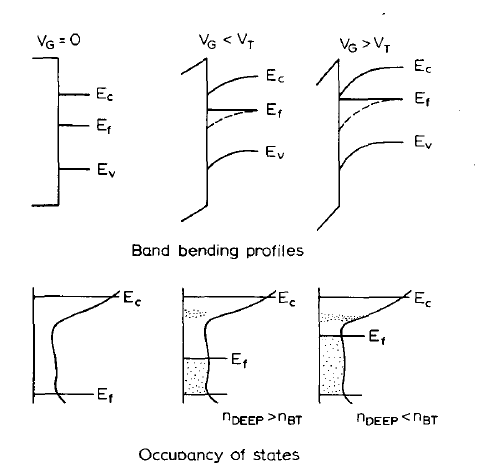
\includegraphics[width=6.0cm]{img/imagen-5.png}}
    \caption{Example of a figure caption.}%
    \label{fig5}
\end{figure} 
    
    Esencialmente, los estados localizados en el silicio amorfo pueden dividirse en dops tipos, 
    estados de cola y estados profundos [16][17]. Los estados de cola son  los estados de la banda de 
    conducción de silicio ampliados y localizados por el desorden para formar una ``cola'' de estados
    localizados justo por debajo del borde de la movilidad de banda de conducción. Los estados profundos
    se originan a partir de los defectos de la red de silicio amorfo. Se crre que estan formado principalmente 
    por enlaces rotos de silicio, que tienen una amplia gama de energias debido a las variaciones en los 
    entornos locales. 
    \\
    A cero volts de compuerta, las bandas de energía se acercan a la condición de banda plana. Para
    voltajes de compuerta positivos, menores que el voltaje de umbral, las   bandas de energía se 
    doblan hacia abajo y el nivel de fermi se mueve a través de los estados profundos, que son entocnes
    ocupados. Al mismo tiempo, parte de la carga espacial se localiza en los estados decola de banda, 
    pero la ocupación de estos estados es baja, ya que están muy por encima del nivel de fermi, 
    por lo que la carga espacial total está dominada por los estados profundos.
    \\
    El aumento de la corriente fuente-drenaje se debe a la pequeña fracción de electrones que 
    estan en la cola de banda por encima del borde de movilidad de la banda de conducción. 
    La carga espacial en los estados profundos aumenta en proporción al aumento del voltaje de compuerta,
    pero la corriente aumenta exponencialmente, a medida que aumenta la flexión de la banda. 
    Si la denisdad de estados profundos entre el nivel de fermi y los estados de cola fuera constante, entonces
    la pendiente de preumbral en la característica de transferencia logarítmica sería aproximadamente
    inversamente proporcional a la raíz cuadrada de la densidad de estados.
    \\
    Por encima del voltaje umbral, la carga espacial en los estados de cola de la banda supera la 
    carga espacial en los estados profundos, aunque el nivel de Fermi sigue estando por debajo de 
    los estados de cola. Ahora, tanto la carga espacial total como la corriente de drenaje aumentan 
    linealmente con el voltaje de compuerta aplicado y tenemos una movilidad de efecto de campo 
    bien definida. La movilidad se activa térmicamente con una energía de activación dada por 
    la anchura de los estados de cola, no por $E_C - E_F$.
    \\
    Las características de transferencia pueden modelarse a partir de la densidad de estados o, 
    a la inversa, la densidad de estados puede determinarse a partir de un análisis de las 
    características de transferencia resolviendo la ecuación de Poisson para la región de 
    carga espacial [18]-[21]. Para hacer esto, es habitual suponer que la densidad de estados 
    es homogénea en todo el a-Si:H y que no hay estados en la superficie. En realidad, hay 
    algunas pruebas de que la densidad de estados no es homogénea [15], y la densidad de 
    estados de deriva refleja, por lo tanto, las contribuciones de la interfaz y del bulto.
    Las mediciones en función de la temperatura proporcionan más información [22]-[24] y 
    proporcionan un método para determinar el voltaje de banda plana [22].

\begin{figure}[htbp]
    \centerline{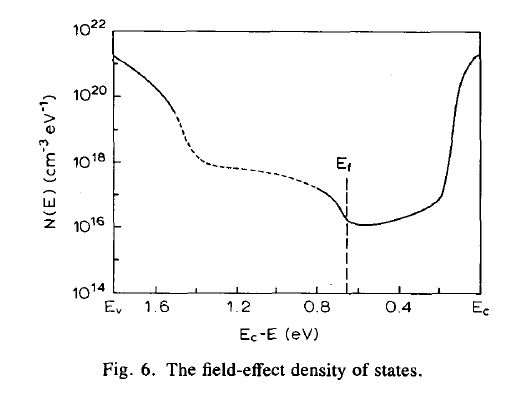
\includegraphics[width=6.0cm]{img/imagen-6.png}}
    \caption{Example of a figure caption.}%
    \label{fig6}
\end{figure} 
    
    La figura 6 muestra la densidad de estados de efecto de campo para el silicio no dopado, 
    que coincide con las características de los transistores fabricados en nuestro laboratorio. 
    El nivel de Fermi está cerca de una región en la que la densidad de estados está disminuyendo, 
    lo que conduce a un fuerte desplazamiento estadístico [23]. Esto proporciona autoconsistencia 
    entre la densidad de estados, la pendiente experimental de preumbral en la característica de 
    transferencia y la dependencia de la temperatura de la conductancia de efecto campo. Los 
    experimentos con transistores de canal n no dan información sobre la densidad de estados por 
    debajo de unos $0,8 eV$, que se deduce por extrapolación (mostrada en la figura 6).
    \\
    El modelo que utilizamos para los estados de cola en la banda de conducción es una cola lineal 
    hasta unos $0,15 eV$ por debajo de $E_C$, con un posible exponencial pronunciado por debajo. 
    Esto se justifica esencialmente por la observación de una movilidad de efecto de campo bien 
    definida en un amplio rango de temperaturas. La energía de activación corresponde a la anchura
    de la región ``linea'' con la movilidad de la banda de electrones libres que es de unos 
    $10 cm^2 V^{-1} s^{-1}$, es decir, al menos un factor de 10 más grande. Una imagen similar 
    de la distribución de los estados de cola se obtiene a partir de un análisis de los resultados 
    de la movilidad de deriva [25],[26]. 
    \\
    Ha habido varios informes de que los estados de cola tienen una distribución de energía 
    exponencial [27], y tal distribución también se ha utilizado en el análisis de las 
    características de TFT[17][28].Esto conduce a una movilidad de efecto campo dependiente de 
    la tensión de compuerta, ya que el nivel de Fermi se mueve hacia los estados de cola [17]. 
    En nuestro modelo, también es posible empujar el nivel de Fermi a los estados de cola, pero 
    esto ocurrirá a voltajes de puerta más altos. La diferencia esencial entre los dos modelos 
    para los estados de la banda de conducción es la inclinación (temperatura característica $T_c$) 
    de cualquier región exponencial y la posición energética en la que la región exponencial cambia 
    a una región lineal. En nuestro modelo, cualquier región exponencial es muy empinada 
    ($T_c \leq  200 K$) o no existe y la transición a una región lineal se produce por debajo 
    del límite de movilidad. En el modelo de cola exponencial, la región exponencial es menos 
    empinada ($Tc \sim 300 K$) y la transición a la región lineal ocurre sólo por encima del 
    borde de movilidad [28].
    \\
    La principal prueba del modelo de cola lineal es la observación de una movilidad de efecto de 
    campo independiente del voltaje de compuerta por encima del voltaje umbral, la movilidad de 
    efecto de campo activada térmicamente [29], la movilidad de deriva activada térmicamente de 
    forma similar [25], y la falta de dispersión significativa en las mediciones de movilidad de 
    deriva de electrones por encima de $200 K$ [25],[26]. Sin embargo, algunos grupos observan 
    un comportamiento diferente y la forma de los estados de cola sigue siendo controvertida.

\section{Características Dinámicas}
    En la mayoría de las aplicaciones, el transistor de película delgada actúa como un interruptor, 
    donde normalmente el transistor se enciende durante decenas de microsegundos y luego se apaga 
    durante decenas de milisegundos. El comportamiento de los transistores en este intervalo de 
    tiempo define las características dinámicas.
    \\
    En primer lugar, consideremos el encendido. Cuando se aplica una tensión de compuerta positiva 
    al electrodo de compuerta, las bandas de energía del silicio descienden, atrayendo electrones 
    a la región del canal desde los contactos de fuente-drenaje. Ahora se producen dos procesos. 
    Está el transporte de los portadores desde los contactos a la región del canal y está el 
    atrapamiento progresivo de los portadores libres en los estados localizados profundos.
    \\
    La carga total en la región del canal se llena hasta un valor igual a $C X V_G$ y este proceso 
    da lugar a una corriente capacitiva que fluye entre la comuerta y los contactos fuente-drenaje. 
    Experimentalmente se encuentra que este transitorio de corriente capacitiva dura aproximadamente 
    $1 \mu s$ para un dispositivo de $10 pm$ de longitud de canal. Después de este periodo, 
    la carga total en el canal es constante, pero la corriente fuente-drenaje continúa disminuyendo 
    hasta $1 s$, debido a la termalización progresiva de la carga en los estados profundos [31].
    \\
    La termalización de los estados profundos tarda más tiempo que el transporte de carga hacia 
    la región del canal, por lo que es posible modelar el encendido mediante un proceso de atrapamiento 
    múltiple unidimensional en la región de flexión de bandas [31]. Es incorrecto suponer el equilibrio
    térmico en la distribución de energía y luego calcular el transporte dentro del canal como 
    hicieron Yue et al. [32].

\begin{figure}[htbp]
    \centerline{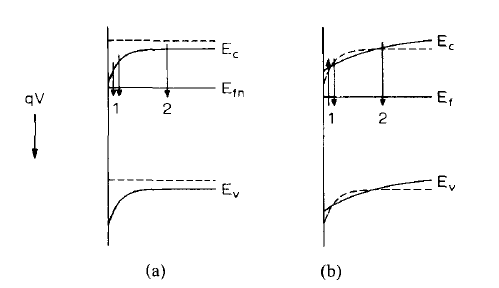
\includegraphics[width=6.0cm]{img/imagen-7.png}}
    \caption{Example of a figure caption.}%
    \label{fig7}
\end{figure} 
    
    La figura 7 ilustra el proceso de termalización. Poco después del encendido (Figura 7(a)), 
    los estados profundos comienzan a atrapar carga, pero la tasa de atrapamiento es mucho mayor 
    cerca de la interfaz del aislante de compuerta (región 1), debido a que la densidad  de 
    portadores libres es mucho mayor, y la ocupación de equilibrio térmico de los estados profundos 
    se establece pronto en esa región. Sin embargo, el atrapamiento de portadores libres en la 
    región 2 continúa, lo que conduce a una transferencia de carga de la región 1 a la región 2 y 
    a un cambio en el perfil de flexión de bandas (Figura 7(b)). Esta redistribución de carga tiene 
    lugar en una escala de tiempo entre $1\mu s$ y $10s$ y conduce a la disminución de la corriente 
    fuente-drenaje observada experimentalmente. La figura 8 muestra el decaimiento experimental de 
    la corriente fuente-drenaje, comparado con el decaimiento calculado utilizando este modelo. 
    El grosor de la capa $i$ era de $3000 A$. La redistribución de la carga entre los estados de 
    cola y los estados profundos puede describirse como un desplazamiento efectivo del voltaje umbral 
    dinámico [31].

\begin{figure}[htbp]
    \centerline{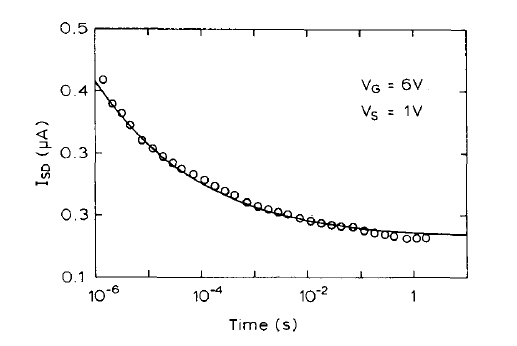
\includegraphics[width=6.0cm]{img/imagen-8.png}}
    \caption{Example of a figure caption.}%
    \label{fig8}
\end{figure} 
    
    El comportamiento de un TFT después de desconectar la puerta se ilustra en la Fig. 9 [33]. Cuando 
    aplicamos una tensión de puerta negativa, las bandas de energía son empujadas hacia arriba y los 
    electrones de la banda son barridos rápidamente hacia los contactos de fuente y drenaje. Después, 
    los electrones comienzan a emitir desde los estados profundos a un ritmo determinado por su 
    profundidad energética. Esto continúa, acumulando una carga espacial uniforme en el silicio amorfo, 
    hasta que la carga espacial positiva en el silicio iguala la carga negativa en la puerta (Figura 9(a)).
    En este punto, se establece el equilibrio térmico en la región 2, pero los estados profundos de la 
    región 1 siguen emitiendo, lo que conduce a una lenta transferencia de carga de la región 1 a la 
    región 2 y, de nuevo, a un cambio en el perfil de flexión de bandas (Figura 9(b)). El proceso de 
    desconexión puede observarse como un decaimiento de la cantidad total de carga almacenada en el 
    dispositivo. En el procedimiento experimental, llamado técnica de descarga[34], la fuente y el 
    drenaje se conectan juntos y medimos la carga almacenada en el dispositivo en función del tiempo, 
    utilizando un electrómetro integrador. La emisión uniforme de carga (Figura 9(a)) conduce a una 
    corriente de descarga y la redistribución de la carga (Figura 9(b)) conduce a otra pequeña corriente 
    de desplazamiento [33]. 

\begin{figure}[htbp]
    \centerline{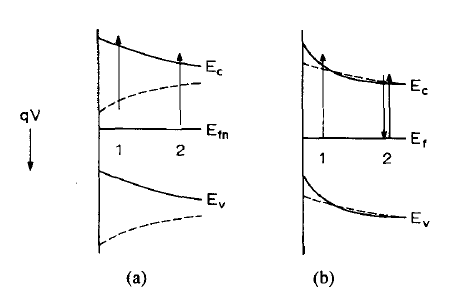
\includegraphics[width=6.0cm]{img/imagen-9.png}}
    \caption{Example of a figure caption.}%
    \label{fig9}
\end{figure} 

    La figura 10 muestra un ejemplo de la caída de la carga en un transistor de película delgada de 
    silicio amorfo, después de la desconexión. El decaimiento presenta claramente dos componentes. 
    El primer componente se debe al establecimiento de una carga espacial uniforme y el segundo se 
    debe a la redistribución de la carga espacial. La flecha de la Figura 10 indica el momento en 
    que en el que la carga espacial en el canal del TFT se iguala por primera vez a la carga en la 
    puerta. Los cálculos de la descarga transitoria utilizando la distribución de la densidad de 
    estados de la Figura 6 muestran un acuerdo razonable con el experimento [33]. En particular, el 
    aumento de la densidad de estados por debajo del nivel de Fermi de banda plana es necesario para 
    obtener tal acuerdo, lo que es un apoyo más para esta imagen de densidad de estados.

\begin{figure}[htbp]
    \centerline{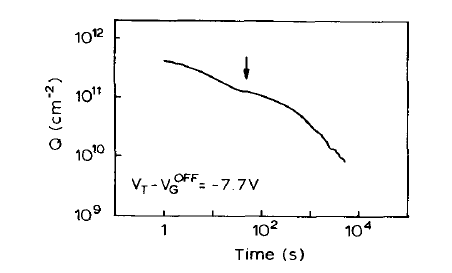
\includegraphics[width=6.0cm]{img/imagen-10.png}}
    \caption{Example of a figure caption.}%
    \label{fig10}
\end{figure} 

    Evidentemente, el proceso de desconexión tarda mucho tiempo antes de que se establezca la 
    situación de equilibrio térmico completo. En la práctica, el equilibrio térmico nunca se 
    establece antes de que el dispositivo se encienda de nuevo. La corriente de apagado es siempre 
    una magnitud dinámica y la corriente medida en una característica de transferencia convencional 
    dependerá de la velocidad de barrido. La diferencia entre ésta y la verdadera corriente de 
    equilibrio depende del grosor de la capa $i$, ya que la corriente se transporta en la región 
    alejada de la interfaz de la puerta.

\section{ESTABILIDAD.}

    Los TFT`s de silicio amorfo presentan algunas inestabilidades. La inestabilidad más importante 
    es el desplazamiento del voltaje umbral que se observa después de una tensión de polarización 
    prolongada (la aplicación de un voltaje de compuerta durante largos períodos). Este efecto se 
    ha estudiado ampliamente, tanto por su importancia práctica como por la visión fundamental que 
    se puede obtener de las propiedades básicas de los materiales amorfos. La Figura 11 muestra la 
    dependencia temporal de la tensión de umbral medida durante 12 décadas de tiempo después de la 
    conmutación en una polarización de puerta de $12 V$. Entre $1 \mu s$ y $1 s$, vemos el 
    desplazamiento dinámico del voltaje umbral, debido a la termalización de los estados profundos, 
    como se ha comentado en la sección anterior. Entre $1$ y $100 s$ el voltaje umbral es 
    esencialmente constante, lo que nos permite definir las características cuasiestáticas. 
    Más allá de los $100 s$, el voltaje umbral comienza a desplazarse de nuevo, y es esta región 
    la que se discute en esta sección.

\begin{figure}[htbp]
    \centerline{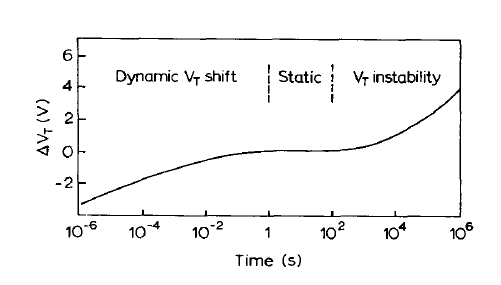
\includegraphics[width=6.0cm]{img/imagen-11.png}}
    \caption{Example of a figure caption.}%
    \label{fig11}
\end{figure} 

    Se han propuesto dos modelos para explicar este desplazamiento del voltaje de umbral, a saber, 
    el atrapamiento de la carga en el aislante de la compuerta de nitruro de silicio [35],[36] 
    y la creación metastásica de nuevos estados en el silicio amorfo [37]-[40]. Estos experimentos 
    fueron capaces de distinguir entre los dos mecanismos y así resolver la verdadera causa del 
    cambio de voltaje umbral. El principio del experimento es el siguiente. Si atrapamos la carga 
    en el nitruro bajo una tensión de polarización positiva, entonces esperamos que el voltaje 
    umbral tanto para la conducción de electrones como de huecos se desplace a valores más positivos. 
    Por otro lado, si creamos estados extra profundos en el a-Si y el nivel de Fermi se mueve a través
    de estos estados para establecer la capa de acumulación de huecos, entonces esperamos que el 
    voltaje umbral para la conducción de huecos se desplace a un valor más negativo, mientras que el 
    voltaje umbral para la conducción de electrones seguirá desplazándose a un valor más positivo. 
    La Figura 12 muestra un resultado experimental para dos voltajes de polarización positivos 
    diferentes: la creación de estados es el mecanismo dominante a $25 V$, pero el atrapamiento de 
    carga domina a 55 V.

\begin{figure}[htbp]
    \centerline{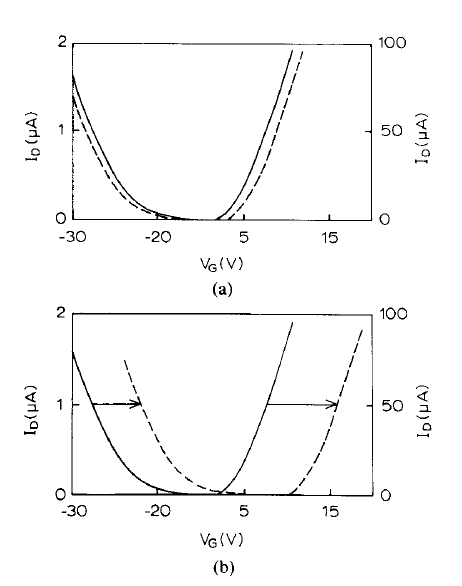
\includegraphics[width=6.0cm]{img/imagen-12.png}}
    \caption{Example of a figure caption.}%
    \label{fig12}
\end{figure} 
    
    La Fig. 13 muestra el desplazamiento del voltaje umbral de los electrones y la contribución a 
    éste de los dos mecanismos en función de la tensión de polarización aplicada $V_{GB}$ [41]. 
    El desplazamiento del voltaje umbral aumenta lentamente con la tensión de polarización hasta 
    el voltaje acrítico $V_{GC}$, a partir del cual aumenta más rápidamente. El desplazamiento del 
    umbral se debe principalmente a la creación de estados por debajo de $V_{GC}$ y al atrapamiento 
    de carga en el nitruro por encima de $V_{Gc}$. El valor de $V_{GC}$ depende del bandgap del 
    nitruro de silicio, lo que confirma que el proceso de captura de carga está relacionado con 
    el nitruro [41]. 

\begin{figure}[htbp]
    \centerline{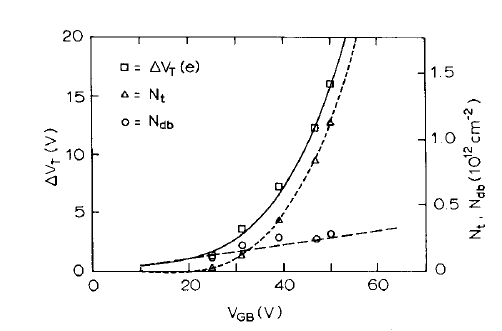
\includegraphics[width=6.0cm]{img/imagen-13.png}}
    \caption{Example of a figure caption.}%
    \label{fig13}
\end{figure} 

    Para el nitruro casi estequiométrico $V_{GC}$ supera los 80 V. El proceso de creación de estado 
    es independiente del nitruro, lo que confirma que la creación de estado tiene lugar tiene lugar 
    en el a-Si [41]. La Figura 14 muestra la dependencia temporal del desplazamiento 
    de la tensión de umbral para un transistor, donde $V_{GC}$ es de unos 50 V, para dos tensiones 
    de polarización diferentes $V_{GB}$ [42]. Los mismos datos se representan en dos escalas 
    diferentes. Para $V_{GB} = 100 V$, domina el atrapamiento de carga y el desplazamiento del 
    voltaje umbral es logarítmico en el tiempo. Para $V_{GB} = 20 V$, domina la creación de estados 
    y el desplazamiento del voltaje umbral viene dado por una dependencia temporal de ley de potencia.
    Además, el desplazamiento del umbral es independiente de la temperatura para el atrapamiento de 
    carga, pero se activa térmicamente para la creación de estado [42].
    
\begin{figure}[htbp]
    \centerline{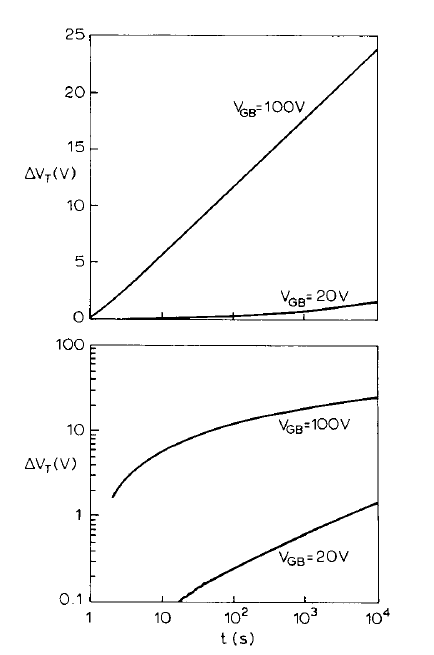
\includegraphics[width=6.0cm]{img/imagen-14.png}}
    \caption{Example of a figure caption.}%
    \label{fig14}
\end{figure} 
    
    La dependencia temporal logarítmica y la independencia de la temperatura se observan generalmente 
    para el atrapamiento de carga en un aislante, donde la corriente de inyección depende 
    exponencialmente de la densidad de la carga previamente inyectada y la carga queda atrapada 
    cerca de la interfaz del aislante de la puerta [43].Esto se observa en los dispositivos MNOS y 
    en varios sistemas MIS, el paso que limita la velocidad es la inyección en el aislante y la 
    conducción en el nitruro es insignificante [42]. Anteriormente habíamos propuesto que la 
    conducción por salto en el nitruro era significativa [35], pero ahora está claro que observábamos 
    el proceso de creación de estado en ese trabajo.

\begin{figure}[htbp]
    \centerline{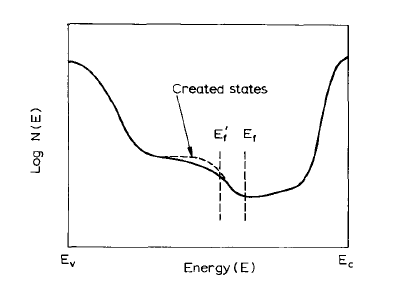
\includegraphics[width=6.0cm]{img/imagen-15.png}}
    \caption{Example of a figure caption.}%
    \label{fig15}
\end{figure} 
    
    El proceso de creación de estado que se observa en los TFT de a-Si tiene varias características 
    en común con las observaciones de creación de estado mediante iluminación o equilibrio térmico[39]. 
    El modelo propuesto es que los enlaces colgantes de Si se crean rompiendo enlaces débiles de 
    Si-Si, que luego se estabilizan por la difusión dispersiva del hidrógeno [44],[45]. La 
    dependencia temporal de la ley de potencia y la dependencia de la temperatura activada 
    térmicamente son consistentes con este modelo [42]. Debido a que la pendiente de preumbral en la 
    característica de transferencia de los transistores de canal n no cambia después de la tensión 
    de polarización, los nuevos estados creados deben estar situados por debajo del nivel de Fermi de 
    banda plana, como se muestra esquemáticamente en la Figura 15. Esto es coherente con la idea de 
    que los estados creados son enlaces colgantes de Si. El proceso de creación de estados anfóteros 
    en esta posición desplazará el nivel de Fermi a un nivel más cercano al de la banda media, lo que 
    explica el desplazamiento del voltaje umbral de los electrones.

\section{FOTOSENSIBILIDAD}

    Los TFT de silicio amorfo son fotosensibles y, sin embargo, para la mayoría de las aplicaciones 
    esto no es deseable. La Figura 16 muestra las características de transferencia de un TFT en 
    la oscuridad y bajo una iluminación superior de $2 \mathsf{X} 10^{4} lux$. La corriente de apagado de 
    $10^{4} A$ es demasiado alta para la mayoría de las aplicaciones.

\begin{figure}[htbp]
    \centerline{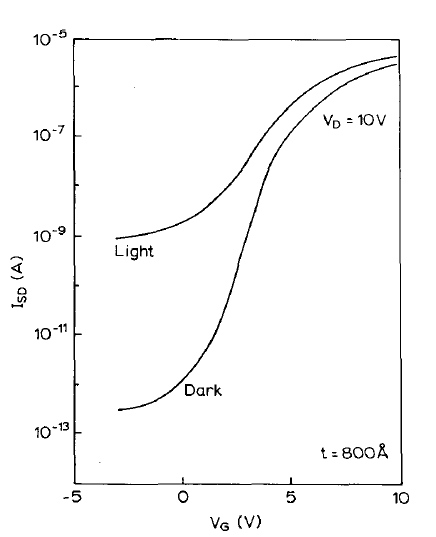
\includegraphics[width=6.0cm]{img/imagen-16.png}}
    \caption{Example of a figure caption.}%
    \label{fig16}
\end{figure} 

    La física básica del efecto fototildado se ha descrito en [46]. Consideremos la generación de 
    pares electrón-hueco en la región de flexión de banda, cuando se aplica una tensión de puerta 
    positiva. Al principio, los electrones son barridos hacia la puerta y los huecos se alejan de 
    la puerta. La carga espacial en los estados localizados se redistribuirá a través del cambio 
    de ocupación inducido por los portadores libres y la flexión de banda se reducirá. Finalmente 
    se alcanza un estado estacionario con un flujo igual de electrones y agujeros en la misma 
    dirección dirección, pero sin flujo de corriente neto perpendicular a la la interfaz.
    \\
    La Figura 17 muestra un ejemplo de la reducción calculada de la flexión de banda, los perfiles 
    de concentración de electrones y huecos, y el flujo de portadores en la condición de estado 
    estacionario [46]. Obsérvese que el nivel de cuasi-Fermi para los electrones es esencialmente 
    plano, pero el nivel de cuasi-Fermi para los huecos no lo es necesariamente. La forma más 
    fácil de reducir la fotosensibilidad de los TFT es utilizar una fina capa de silicio amorfo 
    intrínseco [14],[47]. Además, en los TFT de escalonamiento invertido, hay un cierto 
    apantallamiento de la luz desde el electrodo de puerta.

\begin{figure}[htbp]
    \centerline{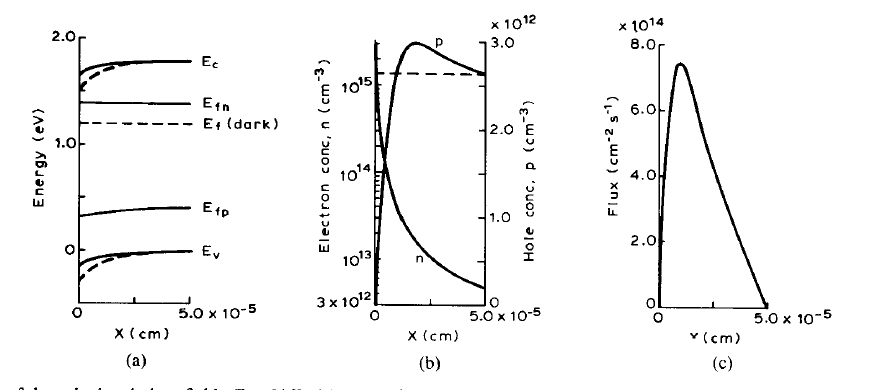
\includegraphics[width=10.0cm]{img/imagen-17.png}}
    \caption{Example of a figure caption.}%
    \label{fig17}
\end{figure}  

    Además, en el caso de un LCD, existe un apantallamiento de la luz desde el otro lado, debido a 
    la máscara negra de la placa de filtro de color [8]. El efecto de apantallamiento de la luz del 
    electrodo de puerta es una de las principales ventajas de la estructura escalonada invertida en 
    comparación con la estructura escalonada normal, en la que a veces es necesaria una capa 
    adicional de apantallamiento de la luz [47].
    \\
    En la Figura 18, mostramos la dependencia del espesor de la capa $i$ de la corriente de salida 
    bajo iluminación, medida a $V_G=- 5 V$ y $V_D= 10 V$, para los transistores de tipo A y de tipo B.
    La iluminación es desde la parte superior (sin apantallamiento de luz), a un nivel de 
    $2 \mathsf{X} 1O^4 lux$ [8]. La corriente de apagado es la misma para ambos tipos de transistores por
    encima de $1000 A$, pero para los transistores de tipo B, disminuye más rápidamente para las 
    capas $i$ más delagadas, mostrando una dependencia de la ley de potencia de 
    aproximadamente $2.5$ en función del espesor. En el caso de los transistores de tipo A, 
    la ley de potencia se sitúa en torno a $1$, lo que puede explicarse sencillamente por la 
    menor absorción y generación óptica en las capas $i$ más finas. 
   
\begin{figure}[htbp]
    \centerline{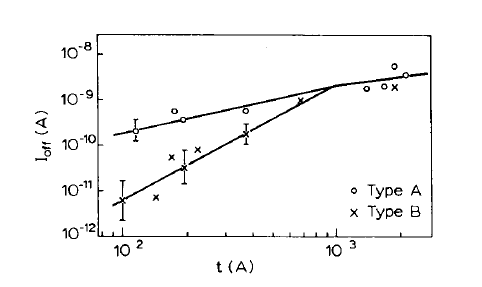
\includegraphics[width=6.0cm]{img/imagen-18.png}}
    \caption{Example of a figure caption.}%
    \label{fig18}
\end{figure}  
 
    Sin embargo, interpretamos 
    que la mayor dependencia del espesor en los transistores de tipo B se debe a una mayor densidad 
    de centros de recombinación en la interfaz superior con el nitruro de silicio. A medida que 
    se reduce el grosor de la capa $i$, estos centros tienen un efecto proporcionalmente mayor 
    en la eliminación de la fotocorriente, por lo que la corriente de apagado disminuye más 
    rápidamente de lo que cabría esperar debido únicamente a la reducción de la absorción óptica. 
    Estos resultados apoyan la observación de una alta densidad de estados rápidos en la interfaz 
    superior del nitruro [48]. Suponemos que estos mismos estados rápidos actúan como centros de 
    recombinación.
    
\begin{figure}[htbp]
    \centerline{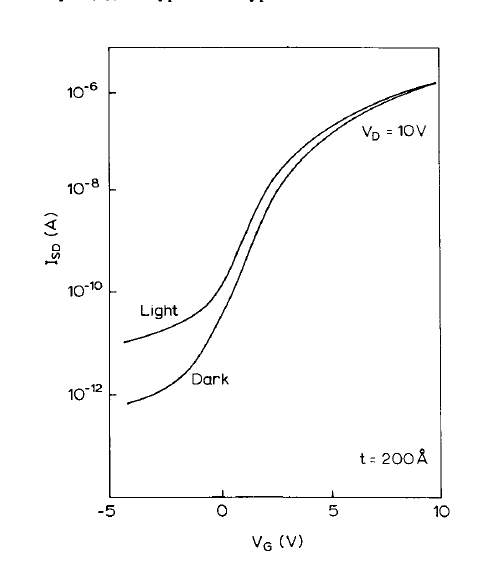
\includegraphics[width=6.0cm]{img/imagen-19.png}}
    \caption{Example of a figure caption.}%
    \label{fig19}
\end{figure} 

    La colocación de una alta densidad de centros de recombinación en la interfase, lejos del 
    aislante de puerta, es la forma óptima de disminuir la fotosensibilidad, con una mínima 
    degradación de la pendiente de pre-umbral en la característica de transferencia. Esto es 
    precisamente lo que ocurre en el transistor tipo B, lo que constituye una ventaja de la 
    estructura tipo B sobre la estructura tipo A. La Figura 19 muestra las características de 
    transferencia, de un transistor tipo B con un espesor de capa $i$ de $200 A$ en las condiciones 
    de luz y oscuridad, como en la Figura 16. Esto es típico de un transistor utilizado en nuestra 
    pantalla de cristal líquido [8].

\section{PASIVACION}

    La capa de pasivación que se deposita sobre el TFT altera las características de un transistor 
    de tipo A, ya que la capa de pasivación está en contacto directo con el silicio en el canal. Por 
    el contrario, la capa de pasivación tiene poco efecto en las características del dispositivo de 
    un TFT de tipo B, ya que el nitruro superior separa la capa de pasivación del silicio. Se han 
    comunicado resultados sobre el efecto de las capas de pasivación en las características de los 
    transistores de tipo A para la pasivación con nitruro de silicio [49], [50], óxido de silicio [50] 
    y poliimida [8]. La Figura 20 muestra un ejemplo del efecto de la pasivación por una capa de 
    poliimida en la característica de transferencia de un transistor tipo A. La pasivación altera 
    las características del transistor al modificar las condiciones de la superficie superior y 
    cambiar la densidad de carga fija y/o los estados superficiales rápidos.
    
\begin{figure}[htbp]
    \centerline{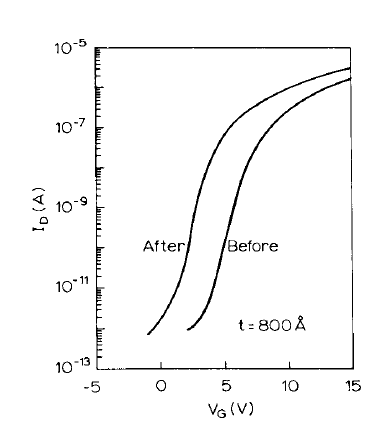
\includegraphics[width=6.0cm]{img/imagen-20.png}}
    \caption{Example of a figure caption.}%
    \label{fig20}
\end{figure} 

    El efecto de los estados rápidos y de la carga fija en la interfaz superior se ha calculado 
    utilizando un programa informático que resuelve la ecuación de Poisson para el efecto de campo, 
    sujeto a las condiciones de contorno adecuadas en la interfaz superior [51].
    Los resultados dependen de la densidad de estados en el a-Si y del grosor de la capa $i$. 
    En el caso de las capas $i$ gruesas o de densidades de estado elevadas, la región de flexión 
    de banda en la interfaz del aislante de puerta y cualquier región de flexión de banda en la 
    interfaz superior, inducida por la carga fija, no interactúan. En este caso, la carga fija 
    aumenta la corriente de desactivación con un efecto insignificante en la tensión de umbral y 
    la movilidad. Sin embargo, en el caso de capas $i$ más finas o densidades de estado bajas, 
    las regiones de flexión de banda interactúan y una carga fija en la superficie superior puede 
    alterar el voltaje umbral [51]. Además, una gran densidad de estados en la superficie superior 
    tenderá a fijar el nivel de Fermi en la interfaz superior y esto hará que el voltaje umbral 
    aumente a medida que el espesor de la capa intrínseca de silicio amorfo disminuya [50].
    





















\end{document}